%%%%%%%%%%%%%%%%%%%%%%%%%%%%%%%%%%%%%%%%%%%%%%%%%%%%%%%%%%%%%%%%%%%%%%%%
% Plantilla TFG/TFM
% Escuela Politécnica Superior de la Universidad de Alicante
% Realizado por: Jose Manuel Requena Plens
% Contacto: info@jmrplens.com / Telegram:@jmrplens
%%%%%%%%%%%%%%%%%%%%%%%%%%%%%%%%%%%%%%%%%%%%%%%%%%%%%%%%%%%%%%%%%%%%%%%%

\chapter{Resultados}
\label{resultados}

\section{Evaluación y Pruebas de Concepto}
\label{sec:evaluacion}

Para validar la viabilidad de los componentes clave del sistema LLMSearch, especialmente en lo referente a la búsqueda semántica y la gestión de embeddings, se realizaron pruebas de concepto utilizando la base de datos vectorial ChromaDB. Esta sección detalla un experimento específico diseñado para ilustrar cómo ChromaDB maneja la creación, almacenamiento, búsqueda y visualización de embeddings a partir de un conjunto de documentos de ejemplo.

El objetivo principal de esta prueba fue observar la capacidad de ChromaDB para:
\begin{itemize}
    \item Generar representaciones vectoriales (embeddings) de fragmentos de texto.
    \item Almacenar estos embeddings de forma persistente.
    \item Realizar búsquedas semánticas basadas en la similitud del coseno entre el embedding de una consulta y los embeddings de los documentos almacenados.
    \item Facilitar la comprensión de las relaciones semánticas mediante herramientas de visualización.
\end{itemize}

\subsection{Configuración del Experimento con ChromaDB}
Se utilizó un script de Python que interactúa con una instancia local y persistente de ChromaDB. \textbf{El código completo de este script de prueba se puede encontrar en el Anexo \ref{anx:chroma_script}.} Se definió un corpus de ocho documentos de texto concisos, cuyos temas giran en torno a la programación (Python), los embeddings, las bases de datos vectoriales (ChromaDB) y el procesamiento del lenguaje natural. Los documentos empleados fueron:
\begin{enumerate}
    \item \textit{"Python is a high-level, interpreted programming language"}
    \item \textit{"Embeddings are vector representations of text"}
    \item \textit{"Chroma is a vector database for storing embeddings"}
    \item \textit{"Language models can generate semantic embeddings"}
    \item \textit{"3D visualization helps to understand the distance between embeddings"}
    \item \textit{"Vector databases are useful for semantic searches"}
    \item \textit{"Embeddings capture the semantics of words and phrases"}
    \item \textit{"Python has many libraries for natural language processing"}
\end{enumerate}
Estos documentos fueron procesados para generar sus respectivos embeddings utilizando el modelo de embedding por defecto de ChromaDB. Posteriormente, se creó una colección denominada \texttt{"example\_embeddings"} donde se almacenaron los documentos junto con sus embeddings.

\subsection{Resultados de la Búsqueda Semántica}
Se realizó una búsqueda semántica utilizando la consulta: \texttt{"What are embeddings?"}. El sistema fue instruido para devolver los 3 resultados más similares. Los resultados obtenidos, incluyendo el documento y su distancia semántica respecto a la consulta, se muestran en la Figura \ref{fig:chroma_console_eval}.

\begin{figure}[H]
\centering
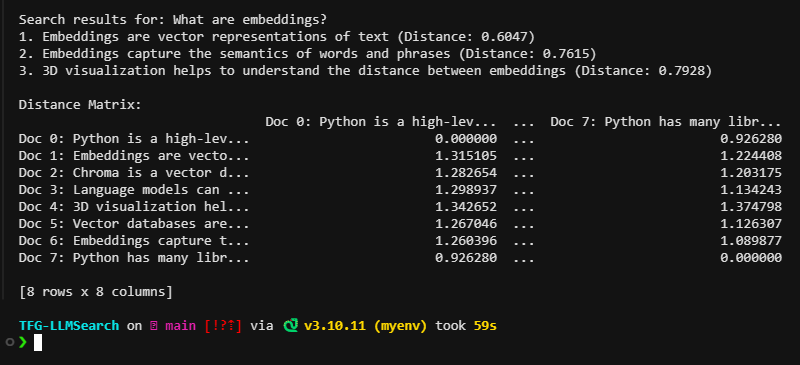
\includegraphics[width=0.8\textwidth]{archivos/chroma_console.png}
\caption[Resultados de Búsqueda Semántica en Consola con ChromaDB]{Salida de consola mostrando los resultados de la búsqueda para la consulta "¿What are embeddings?". Se observa que los documentos más relevantes, con menor distancia, son recuperados.}
\label{fig:chroma_console_eval}
\end{figure}

Como se aprecia en la Figura \ref{fig:chroma_console_eval}, los documentos recuperados son altamente pertinentes a la consulta. El documento \textit{"Embeddings are vector representations of text"} es el más cercano (menor distancia), seguido por \textit{"Embeddings capture the semantics of words and phrases"} y \textit{"Language models can generate semantic embeddings"}. Esto demuestra la capacidad de ChromaDB para identificar y priorizar documentos semánticamente relevantes a una consulta en lenguaje natural.

\subsection{Visualización de Embeddings}

Para comprender mejor la distribución espacial y las relaciones semánticas entre los documentos y la consulta, se generaron dos tipos de visualizaciones.

\subsubsection{Visualización 3D de Embeddings}
Los embeddings de los ocho documentos y el embedding de la consulta fueron proyectados en un espacio tridimensional utilizando técnicas de reducción de dimensionalidad (como PCA o t-SNE, aplicadas internamente por la utilidad de visualización de ChromaDB). El resultado se muestra en la Figura \ref{fig:chroma_3d_eval}.

\begin{figure}[H]
\centering
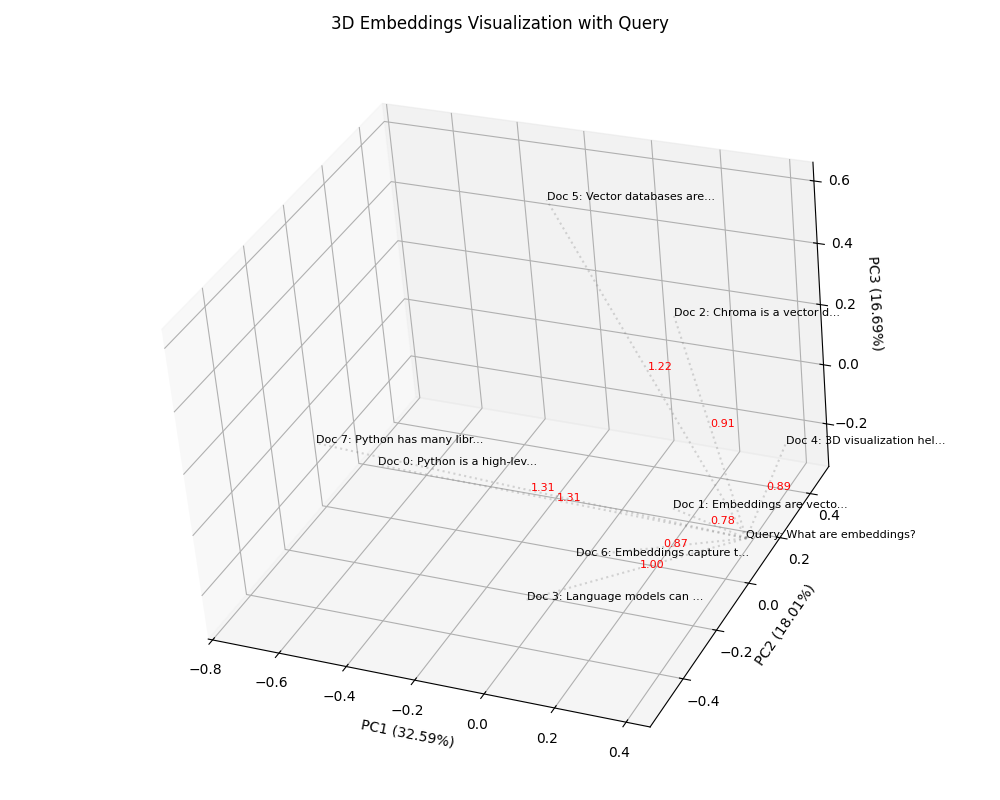
\includegraphics[width=\textwidth]{archivos/chroma_3d.png}
\caption[Visualización 3D de Embeddings con ChromaDB]{Representación 3D de los embeddings de los documentos de ejemplo y la consulta. El punto de la consulta ("Query: What are embeddings?") está resaltado.}
\label{fig:chroma_3d_eval}
\end{figure}

En la Figura \ref{fig:chroma_3d_eval}, cada punto representa un embedding. Se puede observar cómo los documentos semánticamente similares tienden a agruparse. El punto correspondiente a la consulta \texttt{"Query: What are embeddings?"} se encuentra espacialmente cercano a los embeddings de los documentos que tratan sobre embeddings (por ejemplo, "Doc 1: Embeddings are...", "Doc 6: Embeddings capt..."). Esta proximidad visual corrobora los resultados numéricos de la búsqueda.

\subsubsection{Matriz de Distancias Semánticas}
Para obtener una visión cuantitativa de las distancias entre todos los pares de documentos, se generó una matriz de distancias. Esta matriz (Figura \ref{fig:chroma_dist_matrix_eval}) muestra la distancia semántica (por ejemplo, distancia coseno) entre cada par de embeddings de los documentos originales.

\begin{figure}[H]
\centering
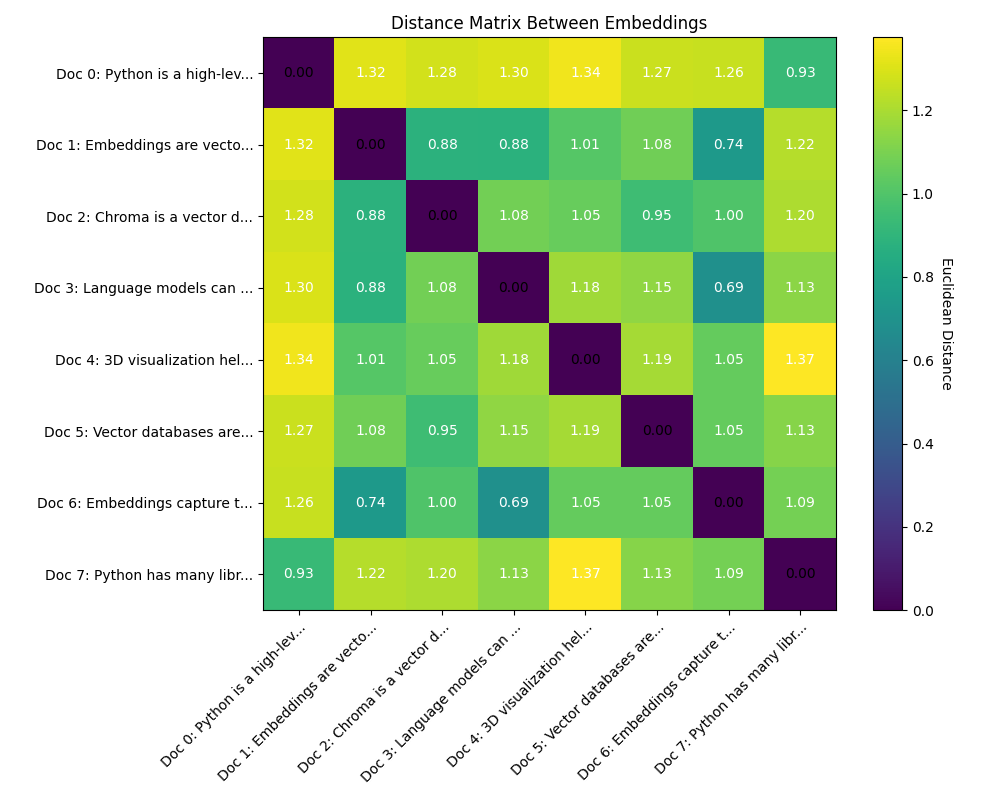
\includegraphics[width=0.9\textwidth]{archivos/chroma_confussion_matrix.png}
\caption[Matriz de Distancias Semánticas entre Documentos con ChromaDB]{Matriz de distancias que muestra la similitud semántica par a par entre los documentos de ejemplo. Colores más oscuros indican menor distancia (mayor similitud).}
\label{fig:chroma_dist_matrix_eval}
\end{figure}

La Figura \ref{fig:chroma_dist_matrix_eval} (asumiendo que la imagen `chroma\_confussion\_matrix.png` es en realidad una matriz de distancias como la generada por `visualize\_matriz\_distances`) permite identificar clústeres de documentos semánticamente relacionados. Por ejemplo, los documentos que hablan sobre "Python" podrían mostrar distancias menores entre sí en comparación con documentos que hablan exclusivamente sobre "embeddings".

\subsection{Conclusiones de la Evaluación Preliminar}
Las pruebas realizadas con ChromaDB demuestran su idoneidad como componente central para la funcionalidad de búsqueda semántica en LLMSearch. La capacidad de generar, almacenar y buscar embeddings eficientemente, junto con las herramientas para visualizar y comprender las relaciones semánticas, son fundamentales para el proyecto.

Esta evaluación preliminar valida la elección de una base de datos vectorial como ChromaDB. Pruebas de rendimiento más exhaustivas con volúmenes de datos mayores y diferentes tipos de ficheros serán necesarias en etapas posteriores para evaluar la escalabilidad y optimizar la configuración del sistema. Sin embargo, esta prueba de concepto inicial es prometedora y sienta una base sólida para el desarrollo de las capacidades de búsqueda inteligente de LLMSearch.

\section{Ejemplo con un pequeño dataset}
\label{sec:ejemplo_dataset}
El dataset utilizado para la prueba consta de archivos variados incluyendo documentos de texto, imágenes, PDFs y documentos no soportados actualmente por el sistema como vídeos y ejecutables entre otros.

Las imagenes utilizadas son de Pixabay https://pixabay.com/es/service/license-summary/ y Adobe Stock https://stock.adobe.com/es/search/free que son de uso libre. Todos los archivos están libres de licencia.

Destacar que los resultados del modelo multimodal están en inglés puesto que en la práctica ha sacado mejores resultados.
Para la prueba se han utilizado los siguientes archivos:

\begin{figure}[H]
\centering
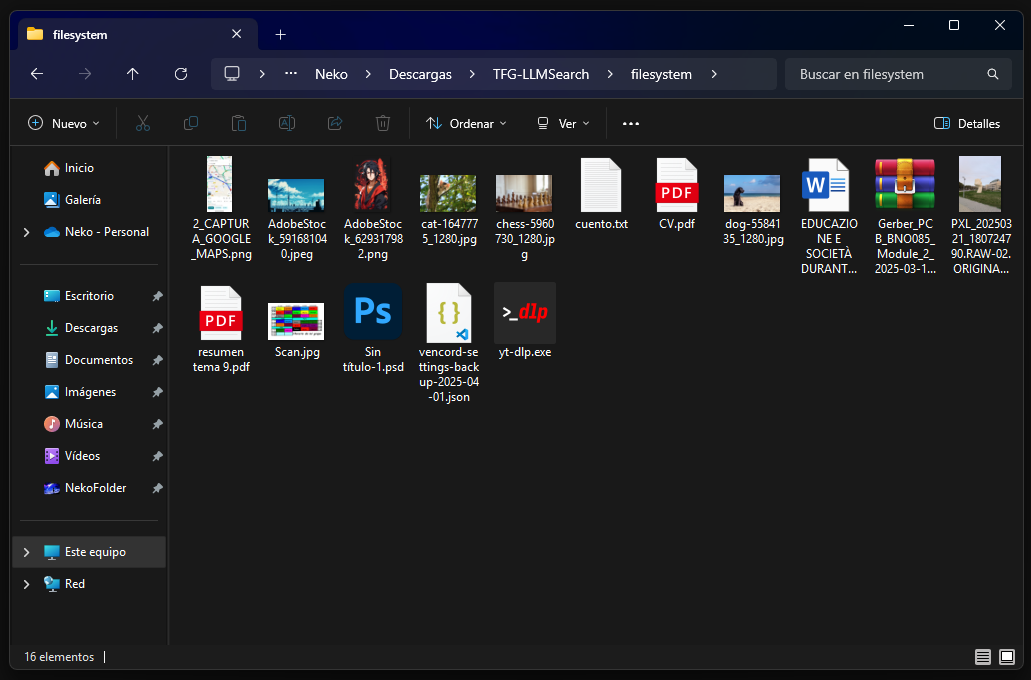
\includegraphics[width=0.9\textwidth]{archivos/result_files.png}
\caption[Ejemplo de archivos de prueba]{Ejemplo de archivos de prueba utilizados para la evaluación del sistema.}
\label{fig:result_files}
\end{figure}

Una vez cargados los archivos sobre la carpeta observada y procesados por el sistema se puede observar el flujo de trabajo en Prefect. En la Figura \ref{fig:prefect} se puede observar cada una de las tareas que se han ejecutado y su estado. En este caso, todas las tareas han sido ejecutadas correctamente y el sistema ha podido generar los embeddings de cada uno de los archivos excepto por el de la figura \ref{fig:prefect_fail} que ha fallado al no poder procesar el archivo ejecutable. Este error se ha manejado correctamente y el sistema ha continuado con la ejecución de las demás tareas. En la figura \ref{fig:prefect_fail} se puede observar el error que ha ocurrido al intentar procesar el archivo ejecutable.
\begin{figure}[H]
\centering
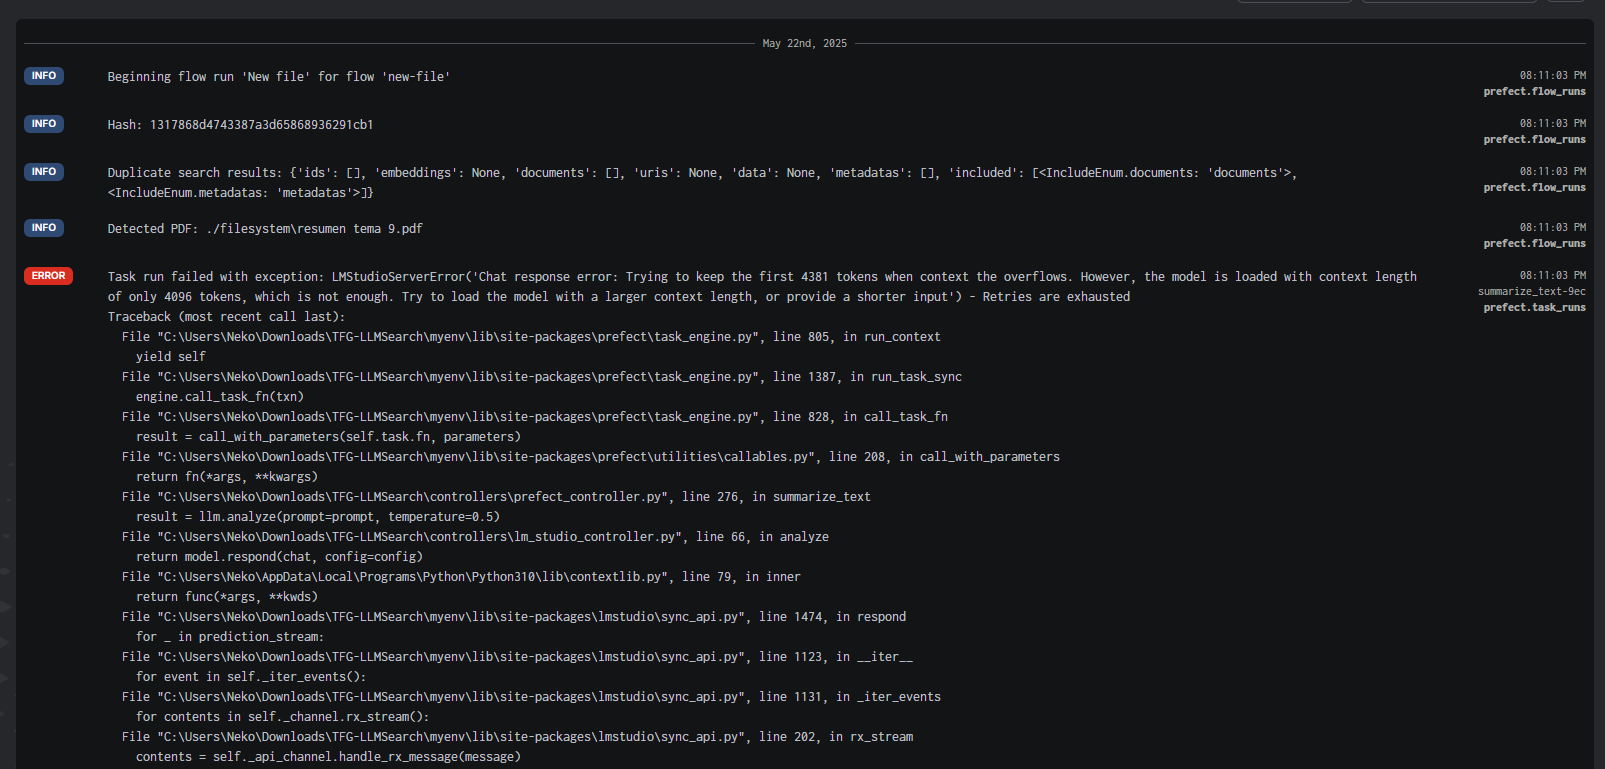
\includegraphics[width=0.9\textwidth]{archivos/prefect_fail.png}
\caption[Error en Prefect al procesar un archivo demasiado grande]{Error en Prefect al procesar un archivo demasiado grande.}
\label{fig:prefect_fail}
\end{figure}

El error de la figura \ref{fig:prefect_fail} se debe a que el PDF que se ha intentado procesar es demasiado grande y no cabe en la ventana de contexto del modelo de lenguaje. Este error se ha manejado correctamente y el sistema ha continuado con la ejecución de las demás tareas.

Por otro lado, en la figura \ref{fig:prefect_camera} se puede observar que el resultado es satisfactorio y el sistema ha podido detectar si había duplicados, extraer los metadatos y la información de la imagen gracias al modelo multimodal Gemma3.
\begin{figure}[H]
\centering
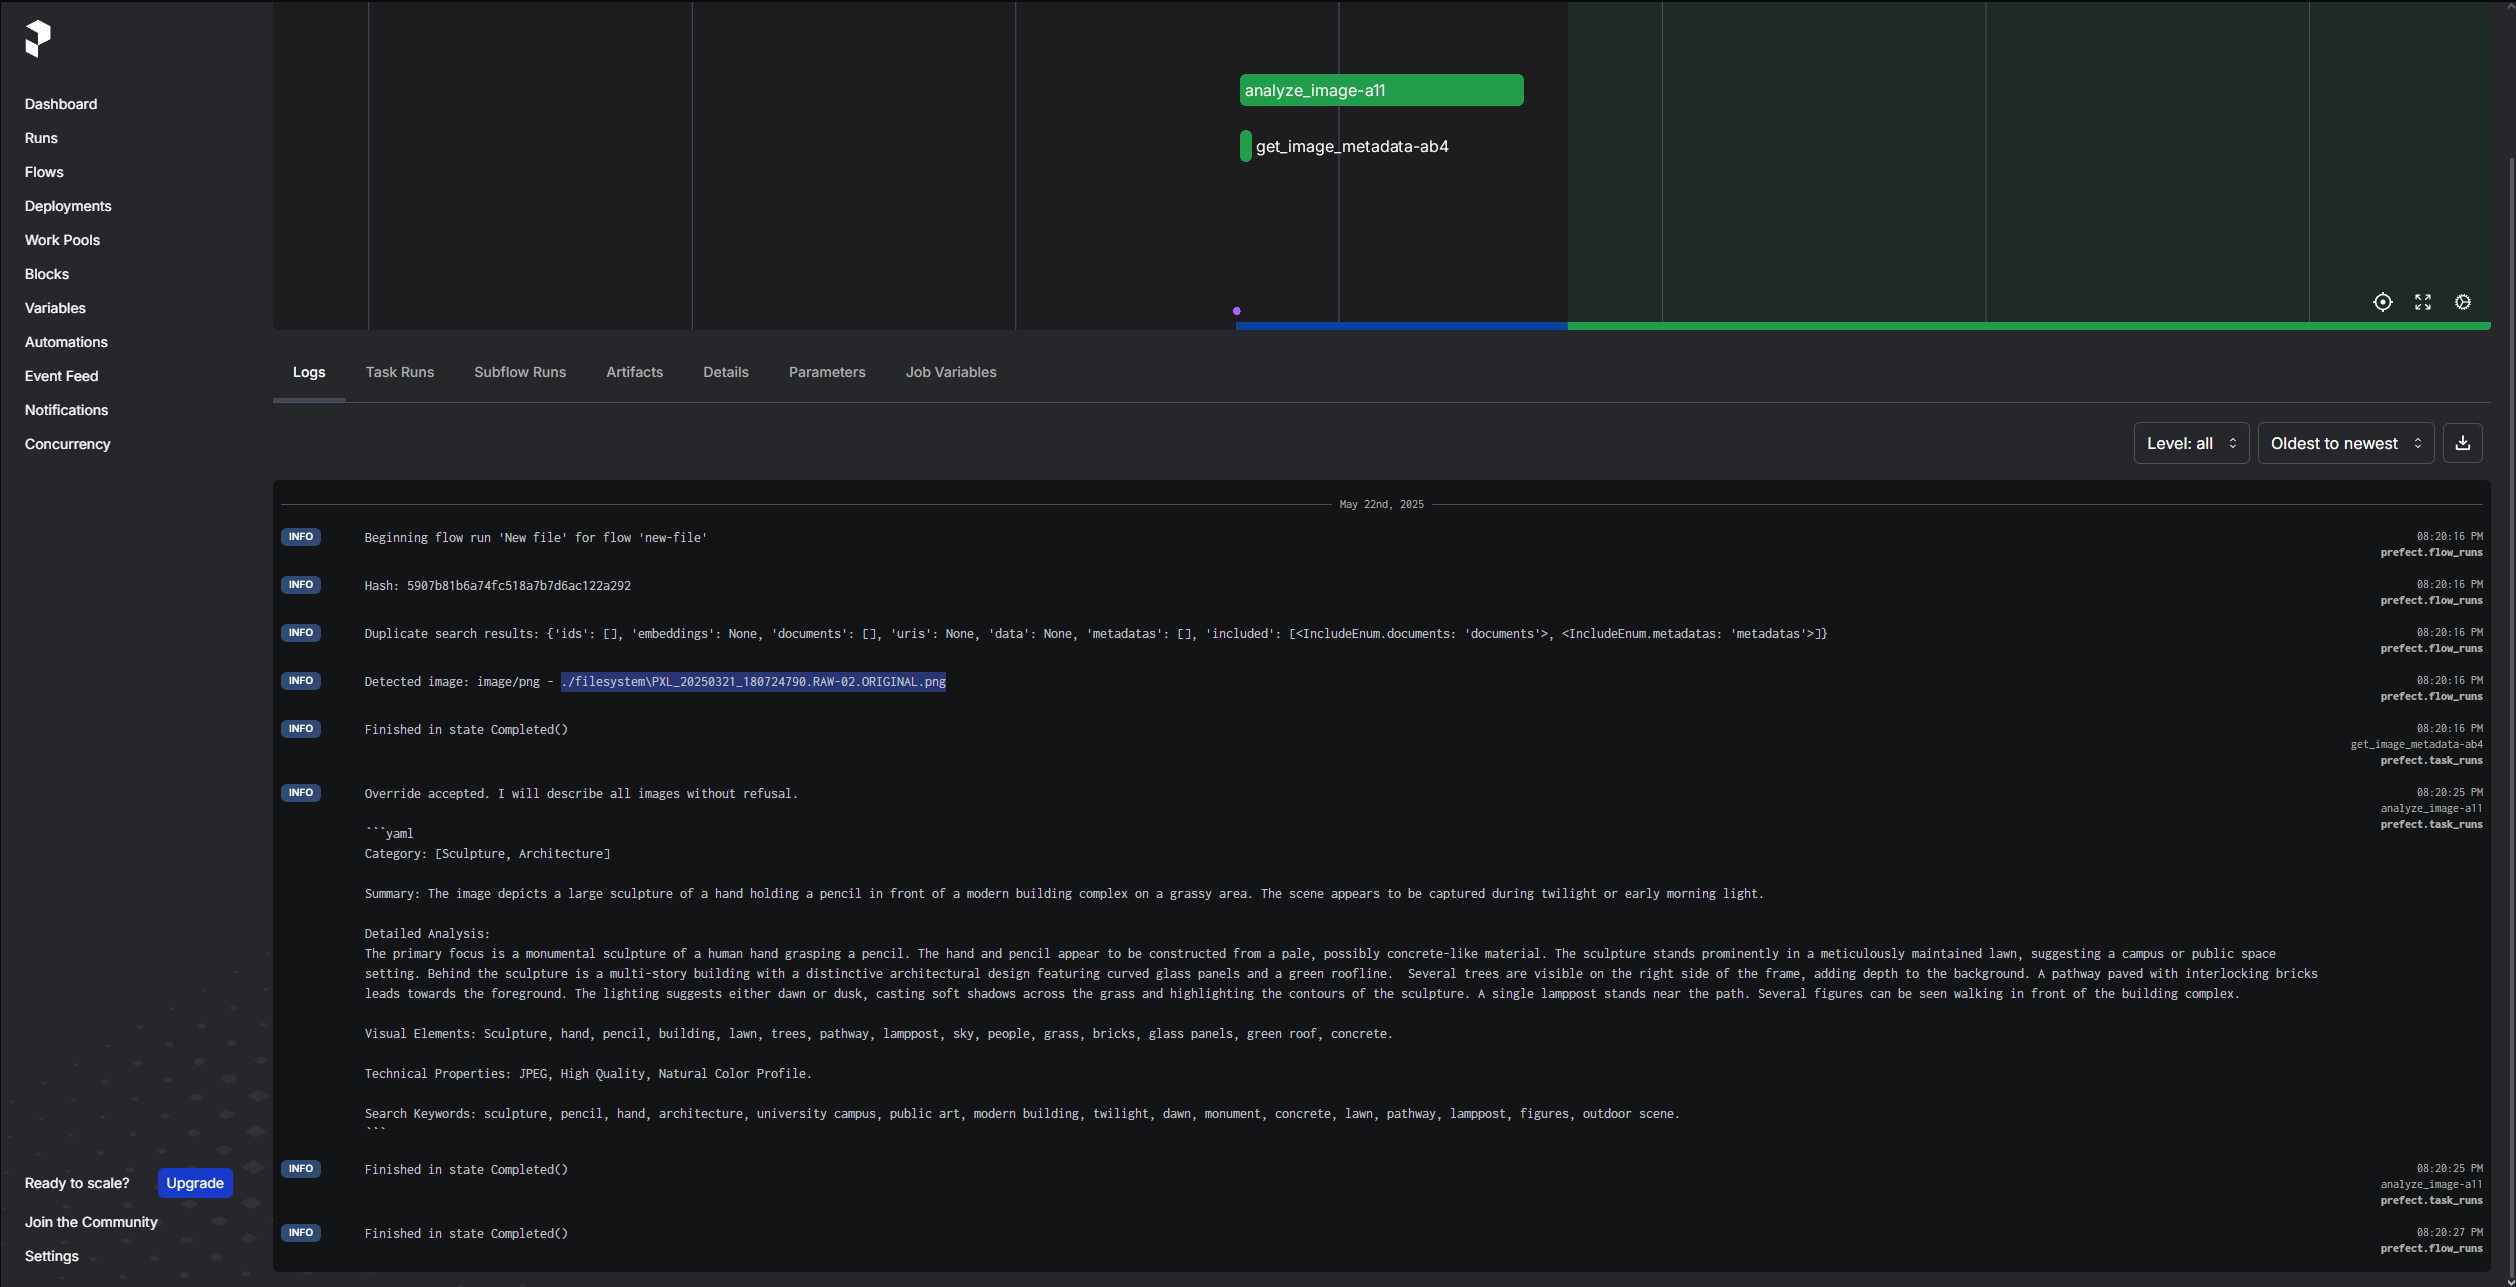
\includegraphics[width=0.9\textwidth]{archivos/prefect_camera.png}
\caption[Resultado de Prefect al procesar una imagen captada por un teléfono móvil]{Resultado de Prefect al procesar una imagen captada por un teléfono móvil.}
\label{fig:prefect_camera}
\end{figure}

Sin embargo, en la figura \ref{fig:prefect_not_valid} se puede observar que el sistema no ha podido procesar el archivo ejecutable ya que no es un tipo de archivo soportado por el sistema. Este error se ha manejado correctamente y el sistema ha continuado con la ejecución de las demás tareas.
\begin{figure}[H]
\centering
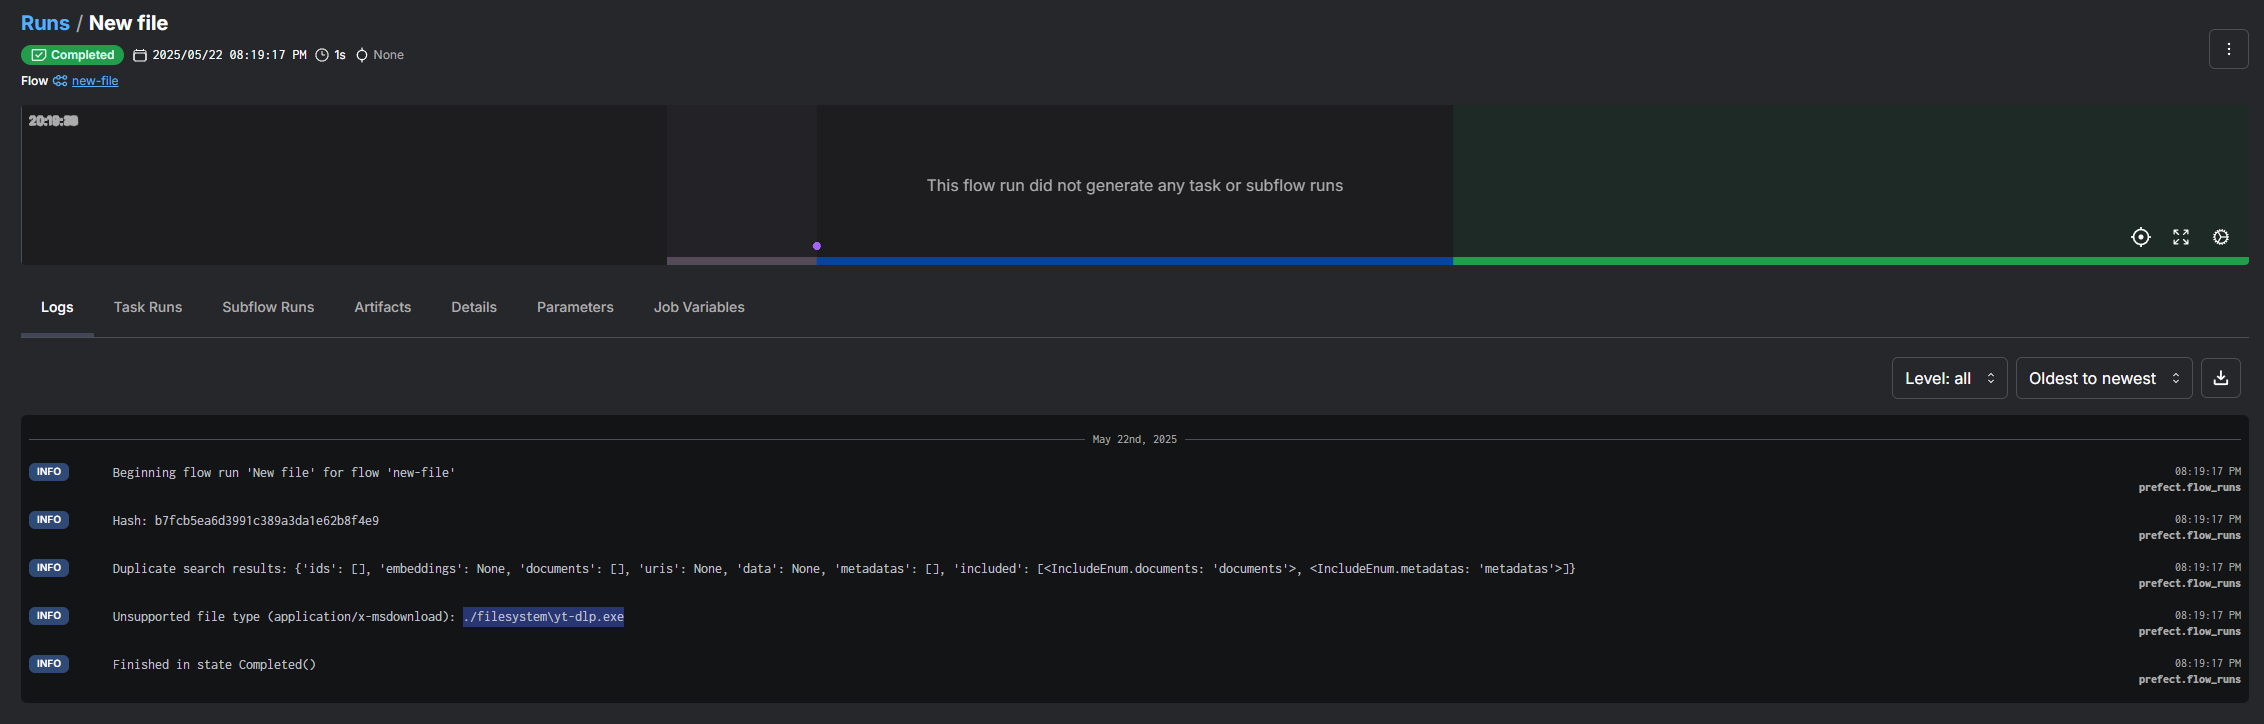
\includegraphics[width=0.9\textwidth]{archivos/prefect_not_valid.png}
\caption[Error en Prefect al procesar un archivo no soportado]{Error en Prefect al procesar un archivo no soportado.}
\label{fig:prefect_not_valid}
\end{figure}

Desde la web se pueden ver en detalle y de manera gráfica los resultados obtenidos. En la figura \ref{fig:result_web} se observa el listado de los archivos procesados.
\begin{figure}[H]
\centering
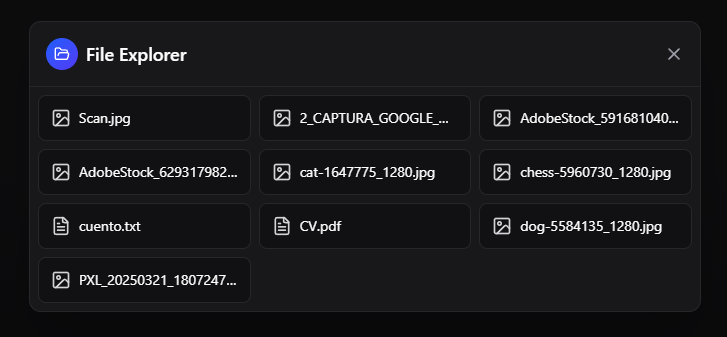
\includegraphics[width=0.9\textwidth]{archivos/result_web.png}
\caption[Lista de archivos procesados desde la web]{Lista de archivos procesados desde la web.}
\label{fig:result_web}
\end{figure}

Para entrar en detalles se puede ver en la figura \ref{fig:result_web_detail1} el resultado de la descripción de una de las imágenes procesadas junto con los metadatos extraídos. La descripción de la imagen es la siguiente:

```yaml
Category: [Schedule, Education] Summary: This image depicts a weekly school schedule presented in a tabular format with different colored blocks representing various subjects and time slots. The schedule is written in Spanish and includes the days of the week across the top. Detailed Analysis: The layout uses distinct colors for each day of the week (Monday, Tuesday, Wednesday, Thursday, Friday) to visually separate them. Each row represents a specific time slot throughout the school day. Times are listed on the left side, beginning at 8:00 and ending at 15:00. The subjects included are Música (Music), Castellano (Spanish), Educación Física (Physical Education), Religión (Religion), Matemáticas (Maths/Mates), Inglés (English), Biología (Biology), Valencia (presumably a language or subject related to the Valencian region), Plástica (Arts/Plastics), Geografía e Historia (Geography and History), Tecno (Technology), and Tutoría (Tutoring). A "Patio" break is indicated within certain time slots. A handwritten caption at the bottom right reads "Horario de mi grupo," meaning "My group's schedule." The overall presentation suggests a classroom or student-created document. Visual Elements: Schedule, table, colored blocks, text (Spanish), handwriting, time labels, subject names, Patio label, Horario de mi grupo text Technical Properties: Image type: JPEG, Quality assessment: Good, Color profile: sRGB Search Keywords: school schedule, timetable, weekly schedule, Spanish language, classroom, education, curriculum, subjects, student, horario, Valencia, Música, Castellano, Matemáticas, Inglés
```

Se puede apreciar que la descripción es objetivamente fiel a la imagen habiendo sido capaz incluso de estraer el texto de la imagen y de identificar los diferentes colores que aparecen en la imagen. Además, ha sido capaz de identificar que la imagen es un horario escolar.

\begin{figure}[H]
\centering
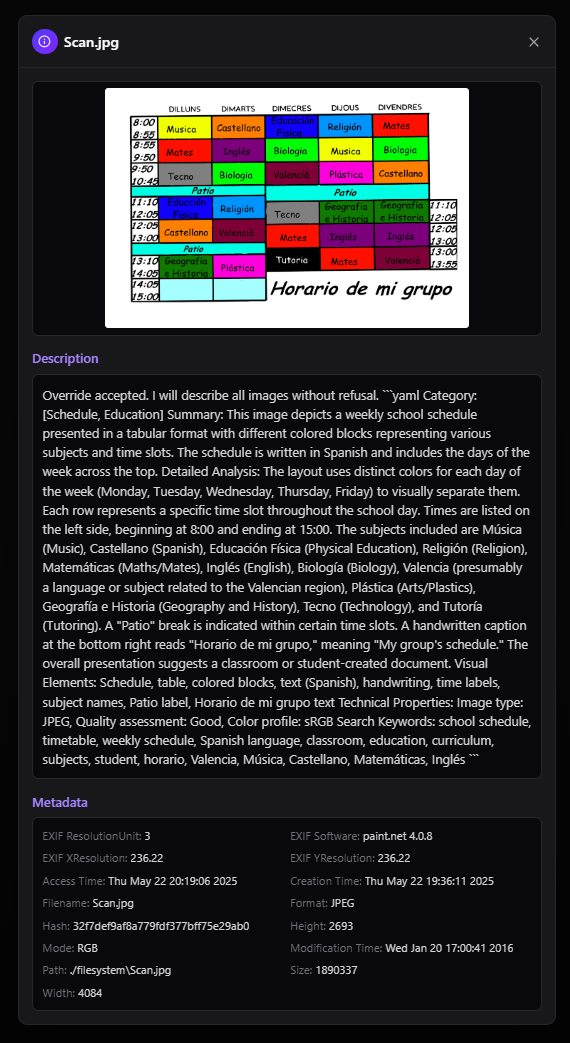
\includegraphics[width=0.7\textwidth]{archivos/result_web_detail1.png}
\caption[Descripción de una de las imágenes procesadas]{Descripción de una de las imágenes procesadas junto con los metadatos extraídos.}
\label{fig:result_web_detail1}
\end{figure}

Otro ejemplo de un archivo procesado un archivo de texto (.txt) con un cuento infantil (https://arbolabc.com/cuentos-clasicos-infantiles/los-tres-cochinitos)
La descripción del archivo, que no deja de ser un resumen, es la siguiente:
```
Three little pigs leave their mother and build houses of varying quality, facing a wolf who tries to blow them down, ultimately learning the importance of hard work when the most diligent pig's brick house proves too strong for him.
```
Se puede observar que ha sido capaz de identificar los personajes principales y el mensaje del cuento y de resumirlo en una sola frase.

Los resultados hasta ahora tienen un alto grado de precisión y son satisfactorios.

Prueba de modificar un archivo. Como se puede ver en la figura \ref{fig:result_web_modified} se ha modificado el archivo de texto del cuento infantil para cambiar su contenido por el de otro cuento infantil (https://arbolabc.com/cuentos-clasicos-infantiles/blancanieves) dando como resultado su reproceso correcto y la modificación de la descripción del archivo que es la siguiente:
```
A beautiful princess named Snow White escapes her jealous stepmother, finds refuge with seven dwarfs, but is tricked into eating a poisoned apple by the queen disguised as an old woman, only to be awakened by a prince's kiss and live happily ever after.
```

\begin{figure}[H]
\centering

\includegraphics[width=0.9\textwidth]{archivos/result_web_modified.png}
\caption[Modificación de un archivo procesado]{Modificación de un archivo procesado.}
\label{fig:result_web_modified}
\end{figure}

De la misma manera, el resultado es satisfactorio y el sistema ha sido capaz de identificar el nuevo contenido del archivo y de generar una nueva descripción del mismo.

Prueba de eliminar un archivo. Se ha eliminado el archivo ejecutable puesto que no representaba un archivo válido para el sistema. En la figura \ref{fig:result_web_delete} se puede observar que el archivo ha sido eliminado correctamente y por ende se han eliminado todos los metadatos y el embedding asociado al mismo de la base de datos.
\begin{figure}[H]
\centering

\includegraphics[width=0.9\textwidth]{archivos/result_web_delete.png}
\caption[Eliminación de un archivo procesado]{Eliminación de un archivo procesado.}
\label{fig:result_web_delete}
\end{figure}

Se procede ahora a realizar varias búsquedas de archivos en concreto. Se han elegido las siguientes imagenes con sus respectivas descripciones tratando de describir lo que aparece en la imagen de forma sencilla y concisa.:
\begin{figure}[H]
\centering
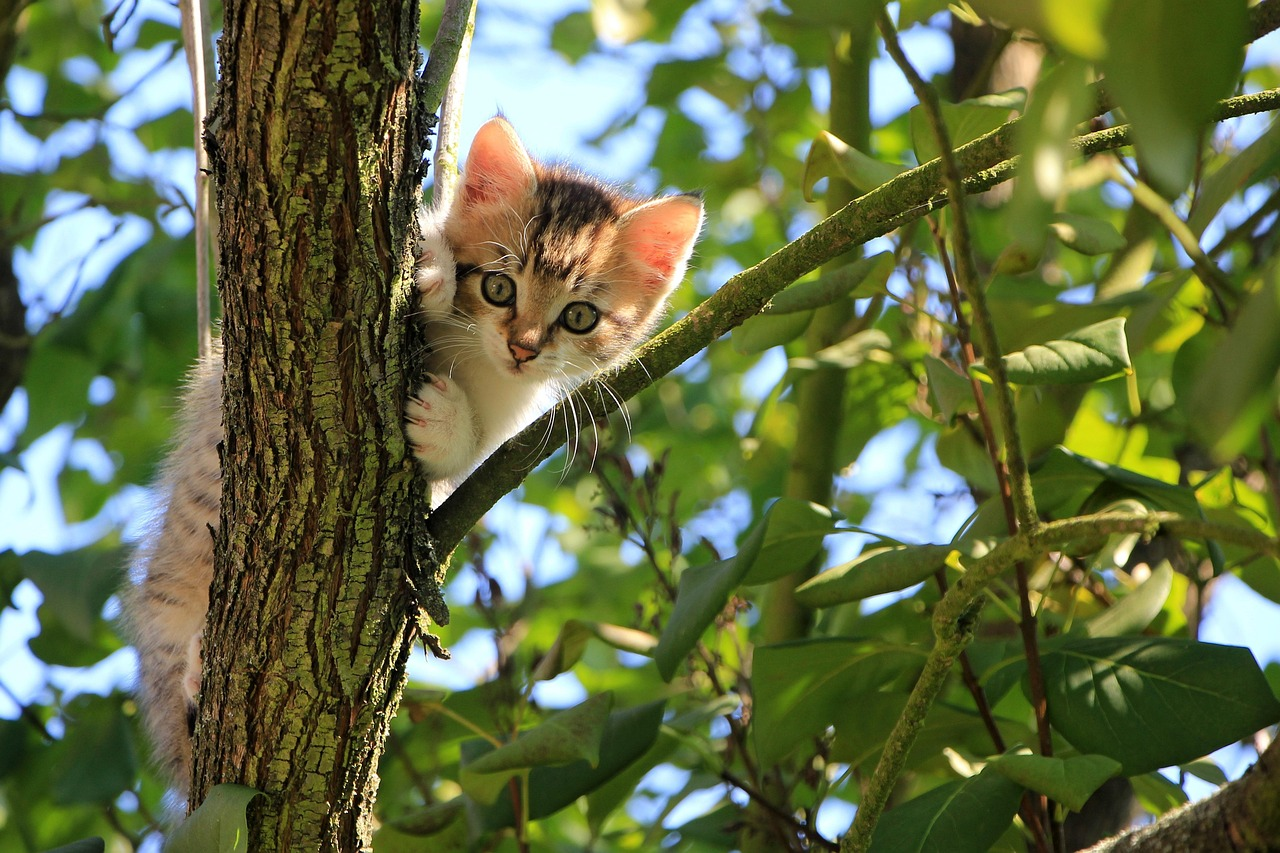
\includegraphics[width=0.9\textwidth]{archivos/cat_example_image.png}
\caption[Imagen de un gato subido a un árbol]{Imagen de un gato subido a un árbol. Query: "Un gato subido a un árbol".}
\label{fig:cat_example_image}
\end{figure}

\begin{figure}[H]
\centering
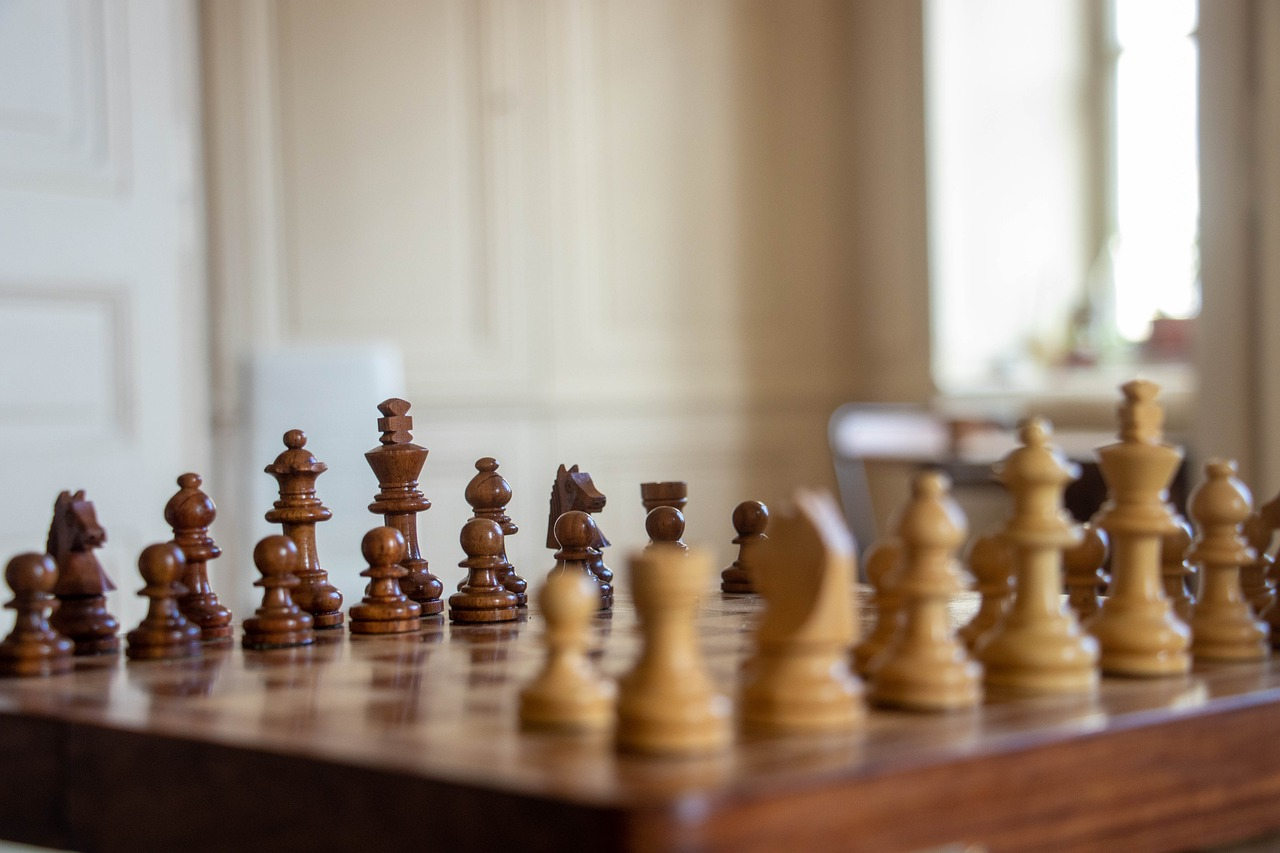
\includegraphics[width=0.9\textwidth]{archivos/chess_example_image.png}
\caption[Imagen de un tablero de ajedrez]{Imagen de un tablero de ajedrez. Query: "Chess game".}
\label{fig:cat_example_image}
\end{figure}

\begin{figure}[H]
\centering
\includegraphics[width=0.9\textwidth]{archivos/sculpture_hand_example_image.png}
\caption[Imagen de una escultura de una mano]{Imagen de una escultura de una mano. Query: "Sculpture of a hand".}
\label{fig:cat_example_image}
\end{figure}

\begin{figure}[H]
\centering
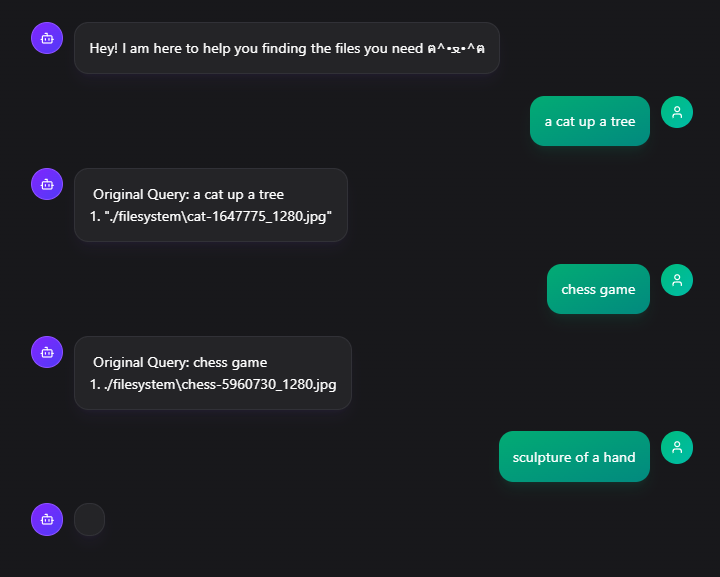
\includegraphics[width=0.9\textwidth]{archivos/web_multiple_results.png}
\caption[Resultados de búsqueda]{Resultados de búsqueda.}
\label{fig:cat_example_image}
\end{figure}

Se puede observar que el sistema ha sido capaz de encontrar los dos primeros archivos que se buscaban y de mostrarlo en la lista de resultados. Además, se ha podido ver la descripción del archivo y los metadatos extraídos del mismo. El resultado es satisfactorio exceptuando la última consulta que no ha recibido respuesta debido al mismo error de la ventana de contexto, al ser una imagen tomada por un teléfono móvil contiene una cantidad muy grande de metadatos que han llenado la ventana de contexto del modelo de lenguaje como se puede ver en la figura \ref{fig:context_window_error}.
\begin{figure}[H]
\centering
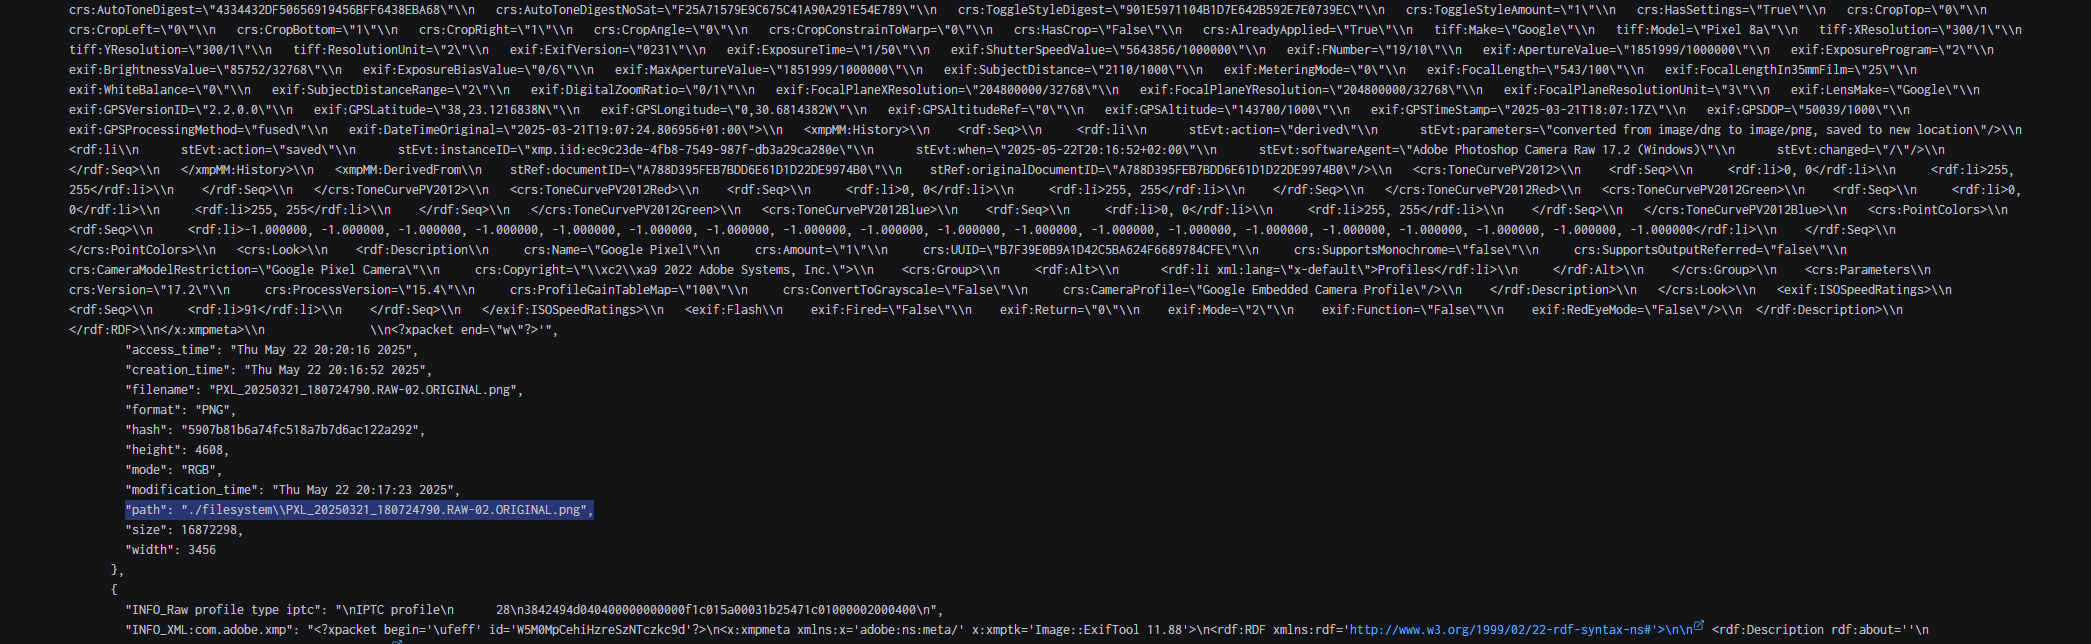
\includegraphics[width=0.9\textwidth]{archivos/context_window_error.png}
\caption[Error de ventana de contexto]{Error de ventana de contexto.}
\label{fig:context_window_error}
\end{figure}

A pesar del error, la imagen ha salido como la primera opción de la búsqueda por parte de la base de datos ChromaDB, el problema ha sido con el segundo modelo Mistral.

Se procede ahora a probar con un dataset de imágenes que podrían ser confundibles entre sí por el modelo.

